\hspace{3mm}

\begin{wrapfigure}{r}{0.35\linewidth}
    \centering
    \includegraphics[width=\linewidth]{VI блок/Киви/lesson_5/Pick's theorem.png}
\end{wrapfigure}

\centerline{\Huge \bf Домашнее задание}
\centerline{\Huge \bf Формула Пика}

\begin{flushright}
    \scriptsize{Пика-пика\\(c) Пикачу}
\end{flushright}

\hspace{3mm}

\problem{1}
Найдите площадь шестиугольника представленного на рисунке справа двумя способами. С помощью формулы Пика и без нее.

\problem{2}
1)\textit{(1 балл)} Хулиган Очир изрезал бумагу листок клетчатой бумаги размером $40\times50$ клетов на 22 многоугольника так, что вершины всех многоугольников лежат в узлах листочка. Ботаник Адьян сосчитал площадь каждого многоугольника и сказал, что они все равны. Прав ли он?

\noindent2) \textit{(2 балла)} На координатной плоскости даны точка $A$ с координатами $(0, 0)$ и точка $B$ с координатами $(m, n)$, где $m, n -$  целые числа. Сколько целых точек находится на отрезке $AB$, включая сами точки $A$ и $B$

\problem{3}
Дана прямая AB, проходящая через те же точки $A$ и $B$, что и во второй задаче. Найдите расстояние от этой прямой до ближайшего к ней узла. 

\problem{4}
Пусть $ABCD$ — квадрат со стороной 1. Точки $P, Q, M, N$ выбраны на его сторонах AB, BC, CD, DA соответственно так, что $AP+AM+CQ+CN = 2$. Докажите, что $AM\perp PQ$

\problem{5}
\textbf{Бонусная задача!} Дана таблица $m\times n$, заполненная целыми числами. За ход Герману разрешается поменять местами две строчки, умножить все числа строчки на $-1$ или же отнять от одной строчку другую, умноженную на некоторое целое число. Те же самые операции можно проводить и над столбцами! Сможет ли он с помощью этих операций добиться вот такой таблицы? Здесь числа $m_1, m_2, \dotsc, m_r$ натуральные, причем каждое следующее делится на предыдущее.

\begin{figure}[h] 
    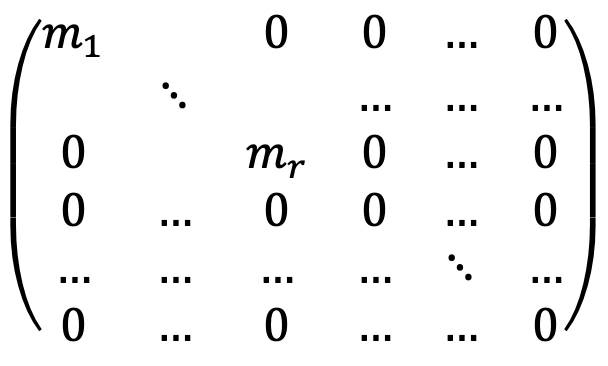
\includegraphics[scale=0.5]{V блок/Киви/lessons_5-6/matrix.png}
\end{figure}